\documentclass{beamer}\usepackage[]{graphicx}\usepackage[]{color}
%% maxwidth is the original width if it is less than linewidth
%% otherwise use linewidth (to make sure the graphics do not exceed the margin)
\makeatletter
\def\maxwidth{ %
  \ifdim\Gin@nat@width>\linewidth
    \linewidth
  \else
    \Gin@nat@width
  \fi
}
\makeatother

\definecolor{fgcolor}{rgb}{0.345, 0.345, 0.345}
\newcommand{\hlnum}[1]{\textcolor[rgb]{0.686,0.059,0.569}{#1}}%
\newcommand{\hlstr}[1]{\textcolor[rgb]{0.192,0.494,0.8}{#1}}%
\newcommand{\hlcom}[1]{\textcolor[rgb]{0.678,0.584,0.686}{\textit{#1}}}%
\newcommand{\hlopt}[1]{\textcolor[rgb]{0,0,0}{#1}}%
\newcommand{\hlstd}[1]{\textcolor[rgb]{0.345,0.345,0.345}{#1}}%
\newcommand{\hlkwa}[1]{\textcolor[rgb]{0.161,0.373,0.58}{\textbf{#1}}}%
\newcommand{\hlkwb}[1]{\textcolor[rgb]{0.69,0.353,0.396}{#1}}%
\newcommand{\hlkwc}[1]{\textcolor[rgb]{0.333,0.667,0.333}{#1}}%
\newcommand{\hlkwd}[1]{\textcolor[rgb]{0.737,0.353,0.396}{\textbf{#1}}}%

\usepackage{framed}
\makeatletter
\newenvironment{kframe}{%
 \def\at@end@of@kframe{}%
 \ifinner\ifhmode%
  \def\at@end@of@kframe{\end{minipage}}%
  \begin{minipage}{\columnwidth}%
 \fi\fi%
 \def\FrameCommand##1{\hskip\@totalleftmargin \hskip-\fboxsep
 \colorbox{shadecolor}{##1}\hskip-\fboxsep
     % There is no \\@totalrightmargin, so:
     \hskip-\linewidth \hskip-\@totalleftmargin \hskip\columnwidth}%
 \MakeFramed {\advance\hsize-\width
   \@totalleftmargin\z@ \linewidth\hsize
   \@setminipage}}%
 {\par\unskip\endMakeFramed%
 \at@end@of@kframe}
\makeatother

\definecolor{shadecolor}{rgb}{.97, .97, .97}
\definecolor{messagecolor}{rgb}{0, 0, 0}
\definecolor{warningcolor}{rgb}{1, 0, 1}
\definecolor{errorcolor}{rgb}{1, 0, 0}
\newenvironment{knitrout}{}{} % an empty environment to be redefined in TeX

\usepackage{alltt}
\usefonttheme[onlymath]{serif}

\usepackage[portuguese]{babel}
\usepackage{graphicx}
\usepackage{ulem} % Para texto em strikeout
\usepackage{amsmath}
\usepackage{amssymb}

\usetheme{m}

\ifdefined\knitrout 
\renewenvironment{knitrout}{\setlength{\topsep}{0mm}}{}
\else
\fi

\title{Aula 4: Modelos Lineares Gerais I}
\subtitle{Análise Quantitativa de Dados Ambientais}
\author{\textbf{Thiago S. F. Silva} - tsfsilva@rc.unesp.br}
\institute{Programa de Pós Graduação em Geografia - IGCE/UNESP}
\date{\today}

\graphicspath{{C:/Users/thiago/OneDrive/UNESP/Pos_graduacao/Eco/2015/Estatistica_2015/Aulas/Aula_4_Regressao_simples/figuras/}}
\IfFileExists{upquote.sty}{\usepackage{upquote}}{}
\begin{document}



%===============================================================================%
\begin{frame}[plain] % plain avoids a badbox error from page number in title page
  \titlepage
\end{frame}

\begin{frame}{Outline}
  \tableofcontents
\end{frame}
%===============================================================================%

\section{Modelos Lineares Gerais}


%===============================================================================%
\begin{frame}{Modelos Lineares Gerais}

Classe de modelos do tipo $\mathbf{Y = BX + U}$, onde $\mathbf{Y}$ é um vetor de respostas, $\mathbf{B}$ é a matriz desenho (\emph{design matrix}), $\mathbf{X}$ é uma matriz de variáveis explicativas, e $\mathbf{U}$ é uma matriz contendo os erros.

\begin{equation*}
\begin{bmatrix}
  y_1\\
  y_2\\
  y_3\\
  . \\
  . \\
  y_n\\
  \end{bmatrix}
=
\begin{bmatrix}
  1 & x_{11} & \dots & x_{1k} \\
  1 & x_{21} & \dots & x_{2k} \\
  1 & x_{31} & \dots & x_{3k} \\
  . & . & . & . \\
  . & . & . & . \\
  1 & x_{n1} & \dots & x_{nk} \\
  \end{bmatrix}
\times
\begin{bmatrix}
  \beta_0 \\
  \beta_1 \\
  \beta_2 \\
  . \\
  . \\
  \beta_k \\
  \end{bmatrix}
+
\begin{bmatrix}
  \varepsilon_1 \\
  \varepsilon_2 \\
  \varepsilon_3 \\
  . \\
  . \\
  \varepsilon_n \\
  \end{bmatrix}
\end{equation*}

\end{frame}
%===============================================================================%

%===============================================================================%
\begin{frame}{Cuidado!}

A nomenclatura é bastante confusa:

\begin{itemize}
  \item General Linear Models (GLM)
  \item Generalized Linear Models (GLM)
  \item Generalized Linear Mixed Models (GLMM)
  \item Generalized Least Squares (GLS)
\end{itemize}

\end{frame}
%===============================================================================%


%===============================================================================%
\begin{frame}
\centering

\only<1-2>{\large{\textbf{Regressão} Linear Simples?}}
\only<3-5>{\large{Regressão \textbf{Linear} Simples?}}
\only<7-8>{\large{Regressão Linear \textbf{Simples?}}}

\vfill

\only<2>{Sir Francis Galton, no século IX, observou que a relação entre alturas de pais e filhos parecia "reverter", ou "regredir" para a média do grupo. A partir dessa observação, Sir Galton desenvolveu uma primeira formulação matemática para a regressão.}

\only<4>{
Os modelos de regressão são formados a partir de combinações lineares de variáveis, através de parâmetros 
\vfill
$Y = \beta _0 +\beta _1 X$ é uma combinação linear de um parâmetro linear $\beta _0$ e um parâmetro linear $\beta _1$ que multiplica $X$ 
\vfill
$Y = \beta _0 +\beta _1 X + \beta _2 X^2$ também é uma combinação linear, de um parâmetro linear $\beta _0$, um parâmetro linear $\beta _1$ que multiplica $X$, e um parâmetro linear $\beta _2$ que multiplica $X^2$
}

\only<5>{

$Y = \beta _0 + e^{\beta _1 X}$ não é uma combinação linear
\vfill
A linearidade se refere aos parâmetros, e não às variáveis
}

\only<6>{

$Y = \beta _0 + e^{\beta _1 X}$ não é uma combinação linear
\vfill
Mas alguns modelos não-lineares podem ser linearizados:
\vfill
$ Ln(Y) = Ln(\beta_0) + \beta_1 X$

$ Z = W + \beta_1 X$

$ Z = Ln(Y)$

$W = Ln(\beta0)$
}

\only<8>{Apenas duas variáveis são usadas, uma dependente ($Y$) e uma independente ($X$)}


\end{frame}
%===============================================================================%



%===============================================================================%
\begin{frame}{Terminologia}
\begin{center}
$Y = \beta _0 + \beta _1 X + \varepsilon$
\end{center}
\vfill
\begin{itemize}
  \item $X$ é a variável \textbf{independente}, também chamada de \textbf{preditor} \pause
  \item $Y$ é a variável \textbf{dependente}, também chamada de \textbf{variável resposta} \pause
  \item $\beta _0$ e $\beta _1$ são os \textbf{parâmetros} ou \textbf{coeficientes} da regressão \pause
  \item $\varepsilon$ é o \textbf{termo de erro}
\end{itemize}  
  
\end{frame}
%===============================================================================%




%===============================================================================%
\begin{frame}{Características de um modelo de regressão}

Os modelos de regressão expressam essencialmente:
\vfill
\begin{itemize}
  \item Uma tendência de $Y$ em variar sistematicamente de acordo com o preditor $X$ \pause
  \item Uma dispersão de pontos ao redor da reta que descreve uma relação estatística  \pause
  \end{itemize}
\vfill
Essas características são expressas através das pressuposições:
\vfill
\begin{itemize}
  \item Existe uma distribuição de probabilidade de $Y$ para cada nível (valor) de $X$ \pause
  \item A média destas distribuições varia sistematicamente com $X$
\end{itemize}  
  
\end{frame}
%===============================================================================%

%===============================================================================%
\begin{frame}{Exemplo}
\centering

\only<1>{
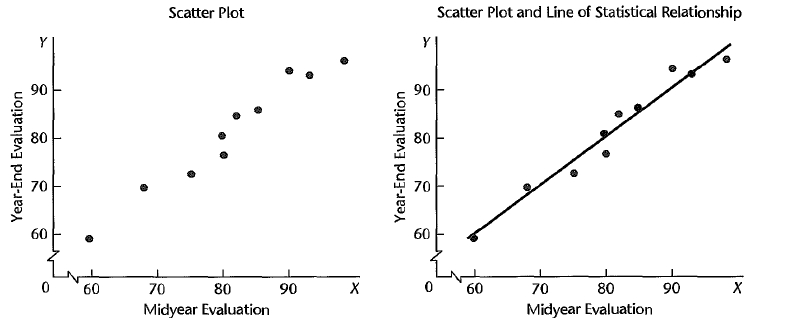
\includegraphics[width=1\linewidth]{Fig_[1].jpg}
}

\only<2>{
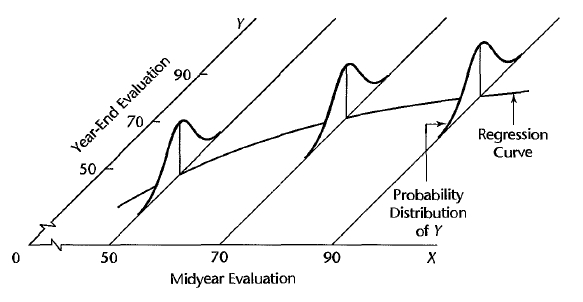
\includegraphics[width=1\linewidth]{Fig_[2].jpg}
}

\end{frame}
%===============================================================================%


%===============================================================================%
\begin{frame}{Regressão e causalidade}

A existência de uma (cor)relação estatística entre duas variáveis não implica em uma relação real de causalidade ou dependência.
\vfill
Mesmo quando há causalidade, cuidado com a direção da relação: $X$ causa $Y$, ou $Y$ causa $X$?
\vfill
\begin{center}
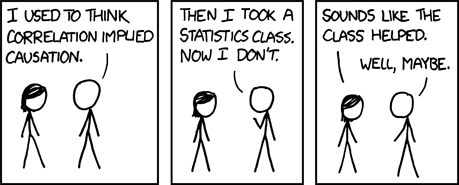
\includegraphics[width=0.7\linewidth]{correlation.png}

\tiny{\url{http://xkcd.com/552/}}
\end{center}

\end{frame}
%===============================================================================%

\section{Formulação do Modelo de Regressão}


%===============================================================================%
\begin{frame}{Formulação do modelo de regressão}

O modelo de regressão completo pode ser escrito como:
\vfill
\begin{center}
$Y_i=\beta _0 + \beta _1 X_i + \varepsilon _i$
\end{center}
\vfill
``O $i$-ésimo valor de $Y$ é função de um parâmetro constante $\beta _0$, somado ao $i$-ésimo valor de $X$ multiplicado por um parâmetro constante $\beta _1$, somado a um $i$-ésimo valor específico de erro''.

\end{frame}
%===============================================================================%


%===============================================================================%
\begin{frame}{Formulação do modelo de regressão}

\begin{columns}[c]

\column{0.5\linewidth}
Se $Y_i$ puder ser predito exatamente por $X_i$, então $\varepsilon _i \sim N(0,0)$
\vfill
$Y_i = 2 + 3X_i$
\vfill
\begin{knitrout}
\definecolor{shadecolor}{rgb}{0.969, 0.969, 0.969}\color{fgcolor}
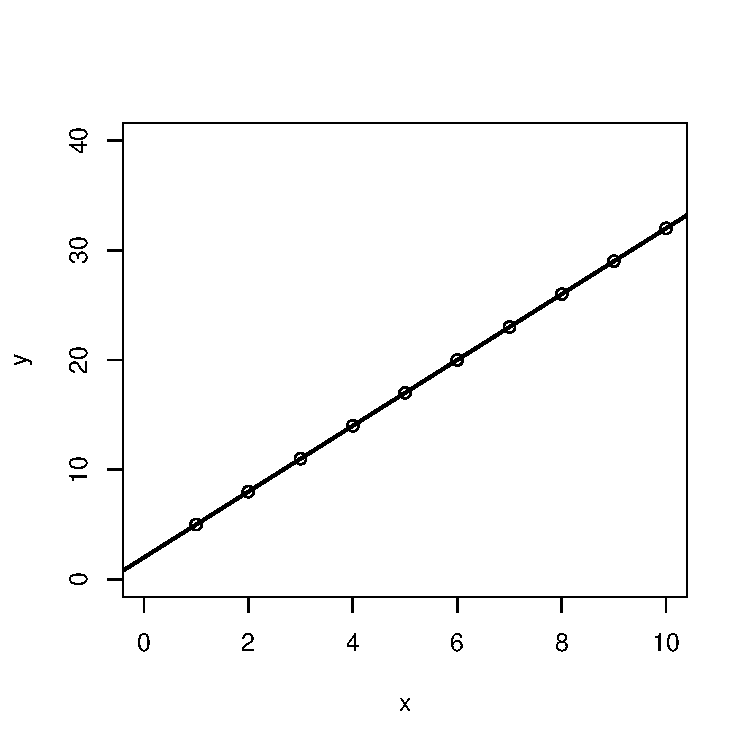
\includegraphics[width=1\linewidth]{figure/ezero-1} 

\end{knitrout}

\column{0.5\linewidth}

\only<1>{
Se $Y_i$ pode ser aproximado por $X_i$, então $\varepsilon_i \sim N(0,\sigma)$
\vfill
$Y_i = 2 + 3X_i + \varepsilon \sim N(0,3)$
\vfill
\begin{knitrout}
\definecolor{shadecolor}{rgb}{0.969, 0.969, 0.969}\color{fgcolor}
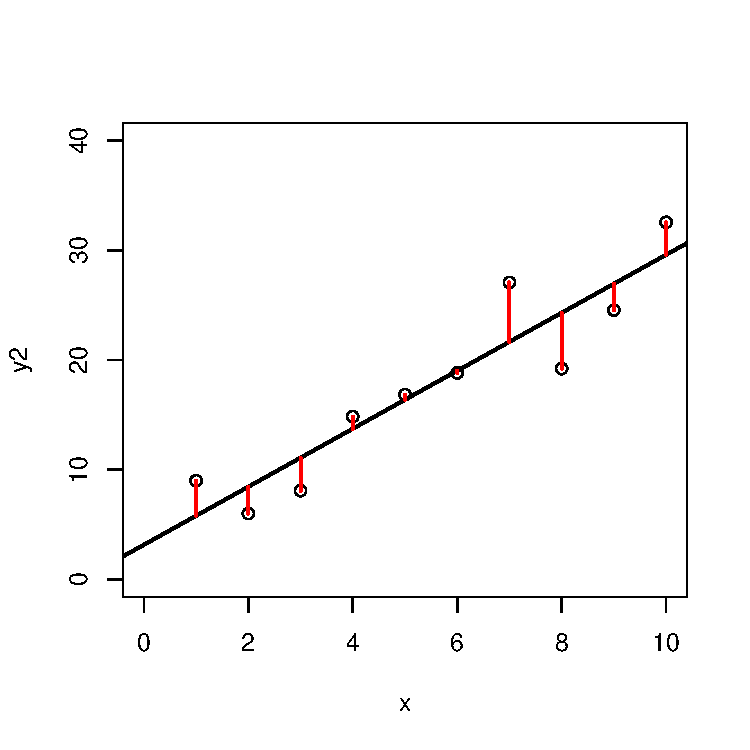
\includegraphics[width=1\linewidth]{figure/enonzero3-1} 

\end{knitrout}
}

\only<2>{
Se $Y_i$ pode ser aproximado por $X_i$, então $\alert{{\varepsilon_i}} \sim N(0,\sigma)$
\vfill
$Y_i = 2 + 3X_i + \varepsilon \sim N(0,6)$
\vfill
\begin{knitrout}
\definecolor{shadecolor}{rgb}{0.969, 0.969, 0.969}\color{fgcolor}
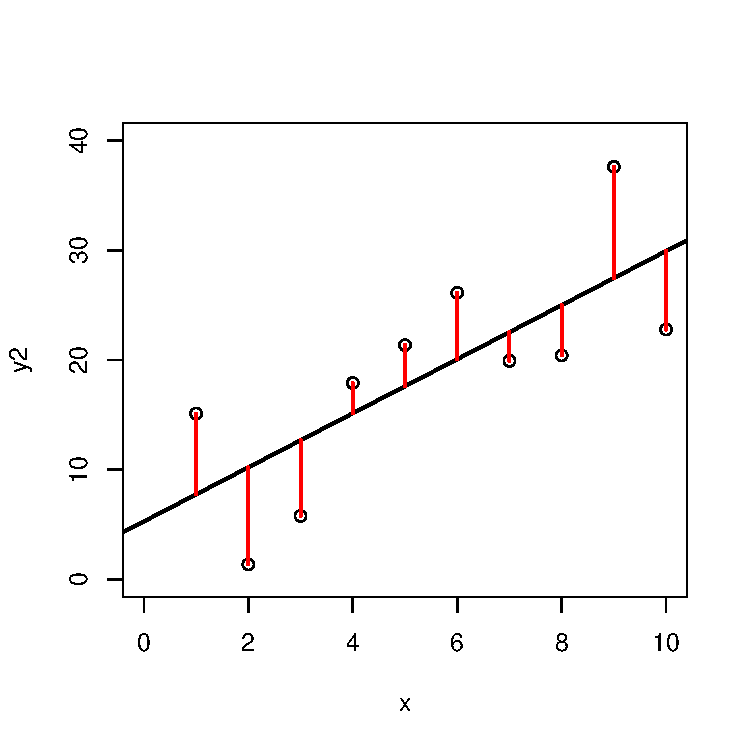
\includegraphics[width=1\linewidth]{figure/enonzero10-1} 

\end{knitrout}
}

\only<3>{
Se ${\varepsilon}$ não possuir média zero, os erros não "regridem" para a linha de tendência central$
\vfill
$Y_i = 2 + 3X_i + \varepsilon \sim N(6,6)$
\vfill
\begin{knitrout}
\definecolor{shadecolor}{rgb}{0.969, 0.969, 0.969}\color{fgcolor}
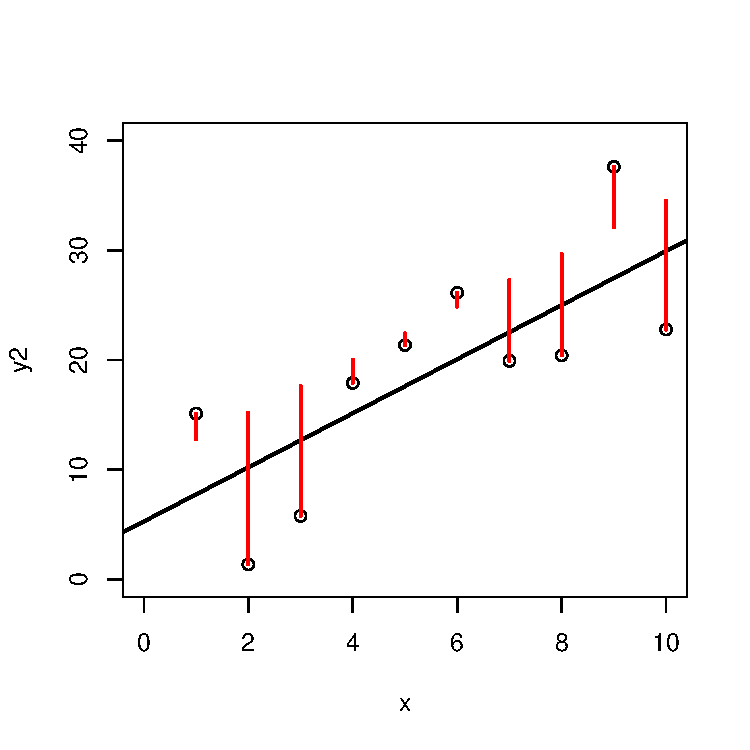
\includegraphics[width=1\linewidth]{figure/enonzero23-1} 

\end{knitrout}
}

\end{columns}

\end{frame}
%===============================================================================%



%===============================================================================%
\begin{frame}{Formulação do modelo de regressão}

Na prática, estamos modelando a \textbf{esperança} de $Y$ para cada nível de $X$:
\vfill
$E[Y_i] = [\beta _0 + \beta _1 X_i + \varepsilon _i]$ \pause
\vfill
$E[Y_i] = \beta _0 + \beta _1 X_i + E[\varepsilon _i]$ \pause
\vfill
Mas nós sabemos que $E[\varepsilon _i] = 0$, então: \pause
\vfill
$E[Y] = \beta _0 + \beta _1 X$

\end{frame}
%===============================================================================%

%===============================================================================%
\begin{frame}{Formulação do modelo de regressão}

Estas relações implicam nas seguintes propriedades:
\vfill
1) $Y_i$ é a soma de um termo constante ($E[Y]$) e um termo aleatório ($\varepsilon$), então $Y_i$ é uma variável aleatória \pause
\vfill
2) A função de regressão para o modelo é $E[Y] = \beta _0 + \beta _1 X$ \pause
\vfill
3) $Y_i$ desvia do valor determinado pela função de regressão por um erro $\varepsilon _i$

\end{frame}
%===============================================================================%


%===============================================================================%
\begin{frame}{Formulação do modelo de regressão}

4) Pressupõe-se que os erros $\varepsilon _i$ tem uma variância constante $\sigma ^2$. Se isso é verdade, $Y_i$ tem a mesma variância:

\vfill
$Var[\beta _0 + \beta _1 X_i + \varepsilon _i] = Var[\varepsilon _i] = \sigma ^2$ \pause
\vfill
$Y_i = \beta _0 + \beta _1 X_i + \varepsilon _i$ \pause
\vfill
$Var[Y_i] = Var[\beta _0 + \beta _1 X_i + \varepsilon _i]$ \pause
\vfill
$Var[Y_i]= \sigma ^2$

\end{frame}
%===============================================================================%

%===============================================================================%
\begin{frame}{Formulação do modelo de regressão}

5) Pressupõe-se que os erros $\varepsilon_i$ são independentes (não-correlacionados). Se quaisquer $\varepsilon _i$ e $\varepsilon _j$ são independentes, então $Y_i$ e $Y_j$ também são independentes:
\vfill
\textbf{Em resumo:} Um modelo de regressão linear simples pressupõe que a resposta $Y_i$ vem de uma distribuição de probabilidade com média $E[Y_i]$ e variância $\sigma ^2$ constante para todos os níveis de X, e que quaisquer $Y_i$ e $Y_j$ são independentes. 

\end{frame}
%===============================================================================%


\section{Os Parâmetros da Regressão}


%===============================================================================%
\begin{frame}{Parâmetros do modelo de regressão}

Os parâmetros ou coeficientes da regressão $E[Y] = \beta _0 + \beta _1 X$ possuem nomes e significados específicos:
\vfill
\begin{itemize}
  \only<2>{\item O parâmetro $\beta _0$ é chamado de ?}
  \only<3-9>{\item O parâmetro $\beta _0$ é chamado de \textbf{intercepto}}
  \begin{itemize}
   \only<4>{\item $\beta _0$ representa ?}
   \only<5-9>{\item $\beta _0$ representa $E[Y_i]$ quando $X = 0$}
   \end{itemize}
\vfill
     \only<6>{\item O parâmetro $\beta _1$ é chamado de ?}
     \only<7-9>{\item O parâmetro $\beta _1$ é chamado de \textbf{inclinação (\emph{slope})} da reta}
  \begin{itemize}
      \only<8>{\item $\beta _1$ representa ?}
      \only<9>{\item $\beta _1$ representa o aumento em  $E[Y_i]$ para um aumento unitário em $X$}
   \end{itemize}
\end{itemize}

\end{frame}
%===============================================================================%

%===============================================================================%
\begin{frame}{Parâmetros do modelo de regressão}
\centering
$E[Y] = 12 + 3X$
\vfill
\begin{knitrout}
\definecolor{shadecolor}{rgb}{0.969, 0.969, 0.969}\color{fgcolor}
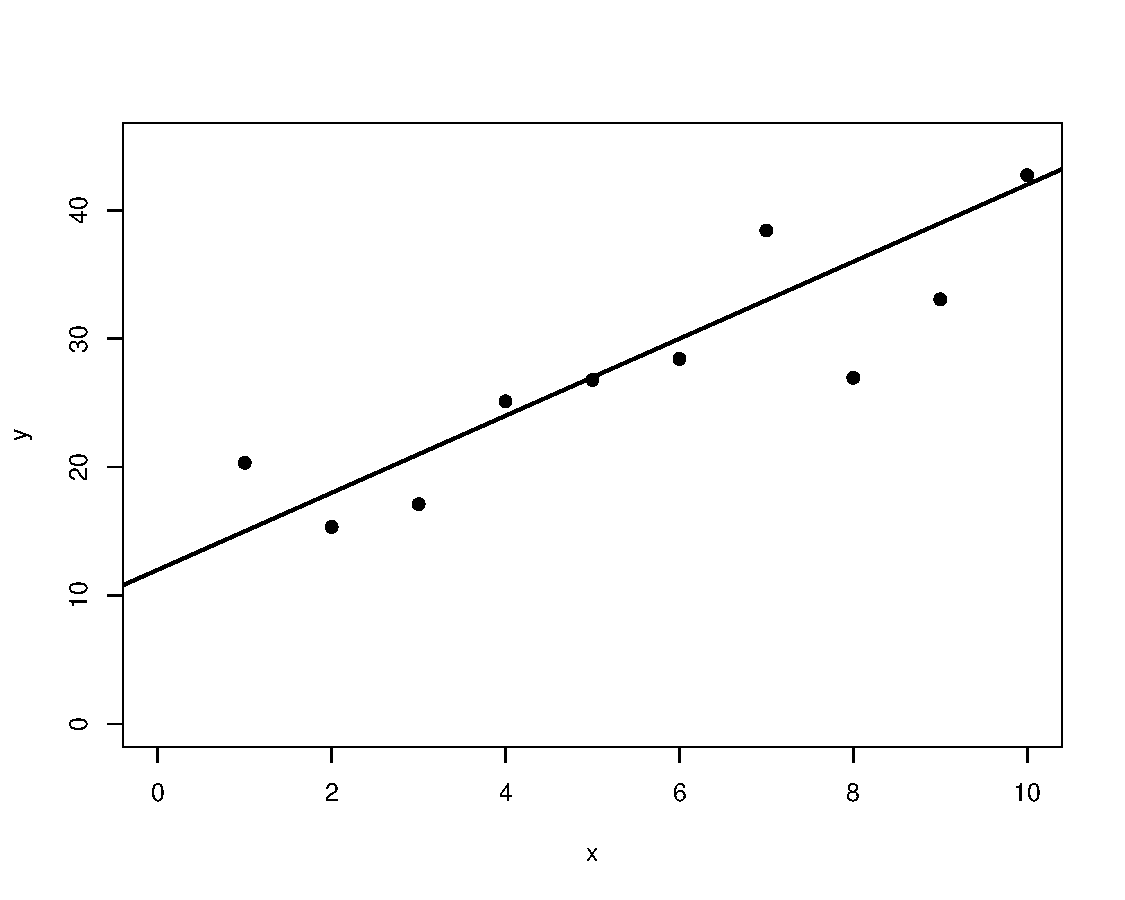
\includegraphics[width=0.7\linewidth]{figure/param1-1} 

\end{knitrout}


\end{frame}
%===============================================================================%

%===============================================================================%
\begin{frame}{Parâmetros do modelo de regressão}
\centering
$E[Y] = 12 + 3X$, $\beta _0 = ?$
\vfill
\begin{knitrout}
\definecolor{shadecolor}{rgb}{0.969, 0.969, 0.969}\color{fgcolor}
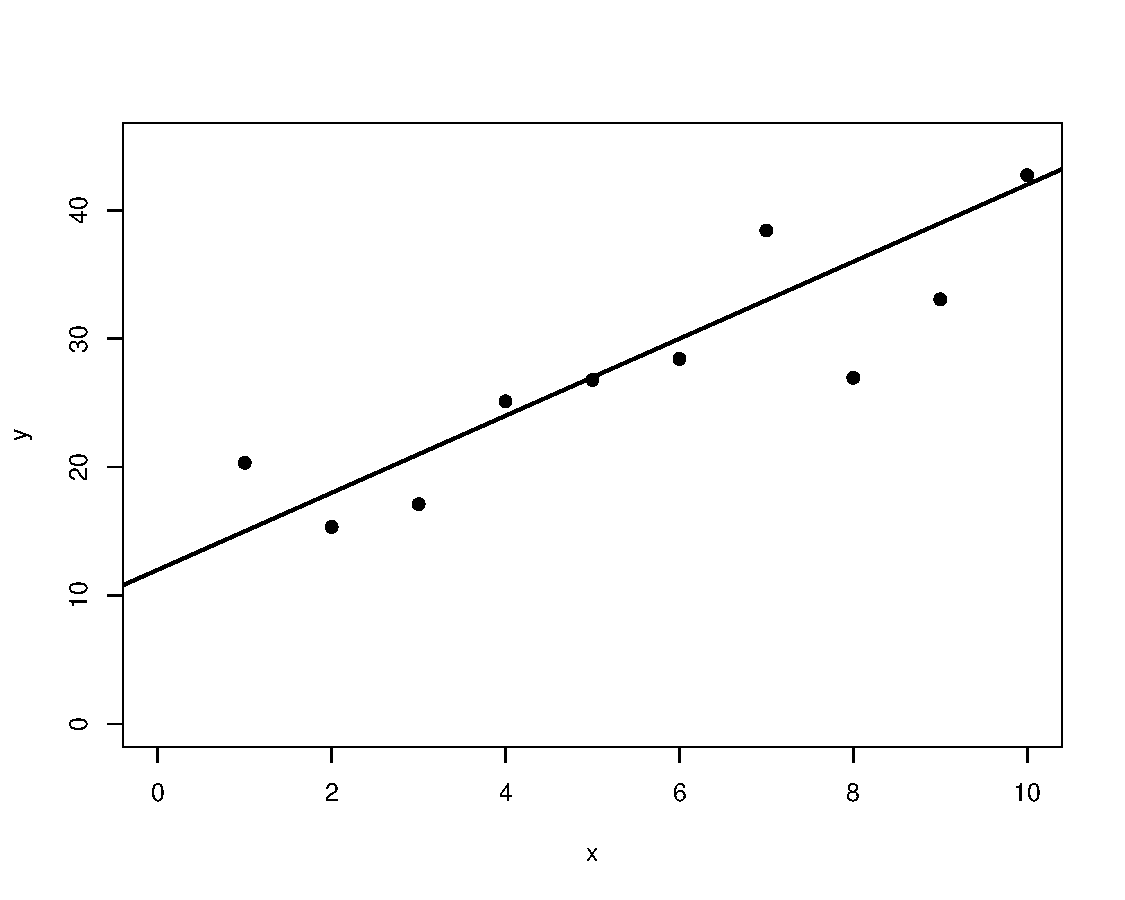
\includegraphics[width=0.7\linewidth]{figure/param2-1} 

\end{knitrout}


\end{frame}
%===============================================================================%



%===============================================================================%
\begin{frame}{Parâmetros do modelo de regressão}
\centering
$E[Y] = 12 + 3X$, \alert{$\beta _0 = 12$}
\vfill
\begin{knitrout}
\definecolor{shadecolor}{rgb}{0.969, 0.969, 0.969}\color{fgcolor}
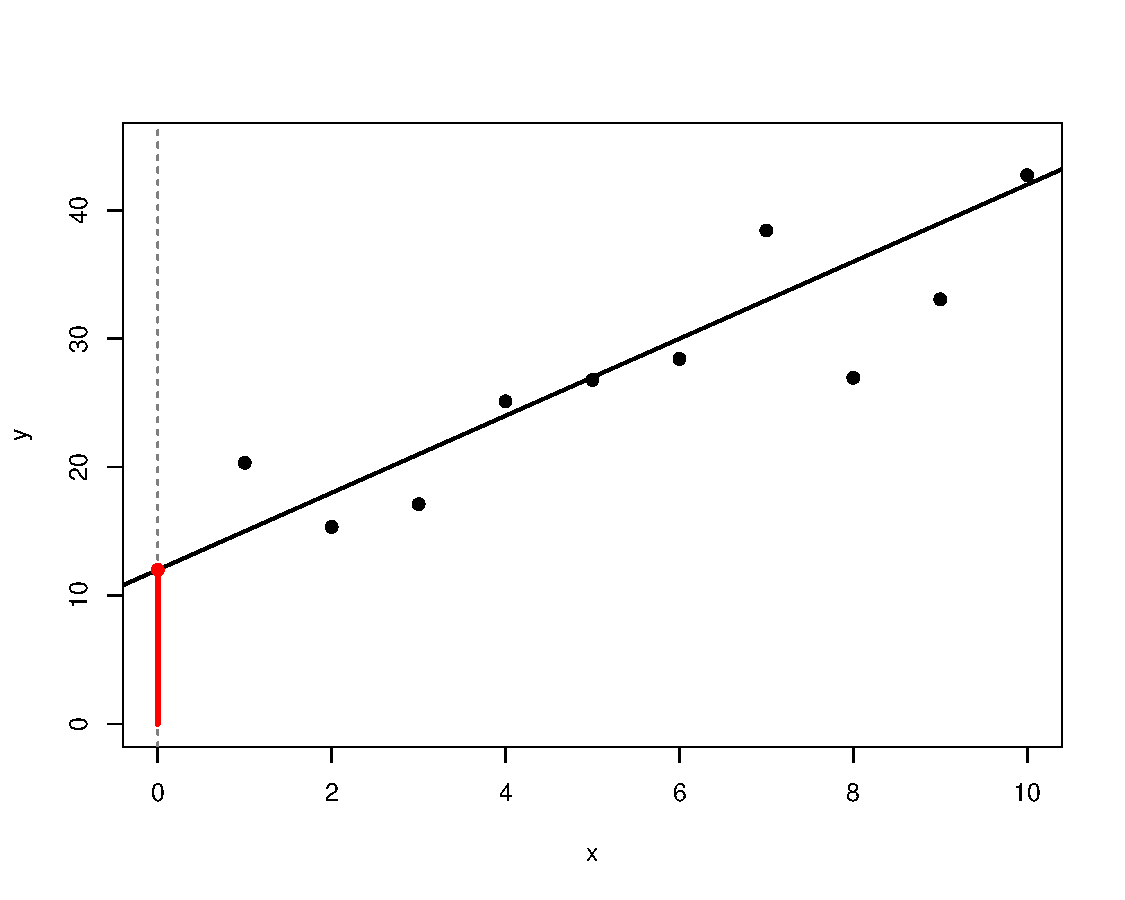
\includegraphics[width=0.7\linewidth]{figure/param3-1} 

\end{knitrout}


\end{frame}
%===============================================================================%


%===============================================================================%
\begin{frame}{Parâmetros do modelo de regressão}
\centering
$E[Y] = 12 + 3X$, $\beta _1 = ?$
\vfill
\begin{knitrout}
\definecolor{shadecolor}{rgb}{0.969, 0.969, 0.969}\color{fgcolor}
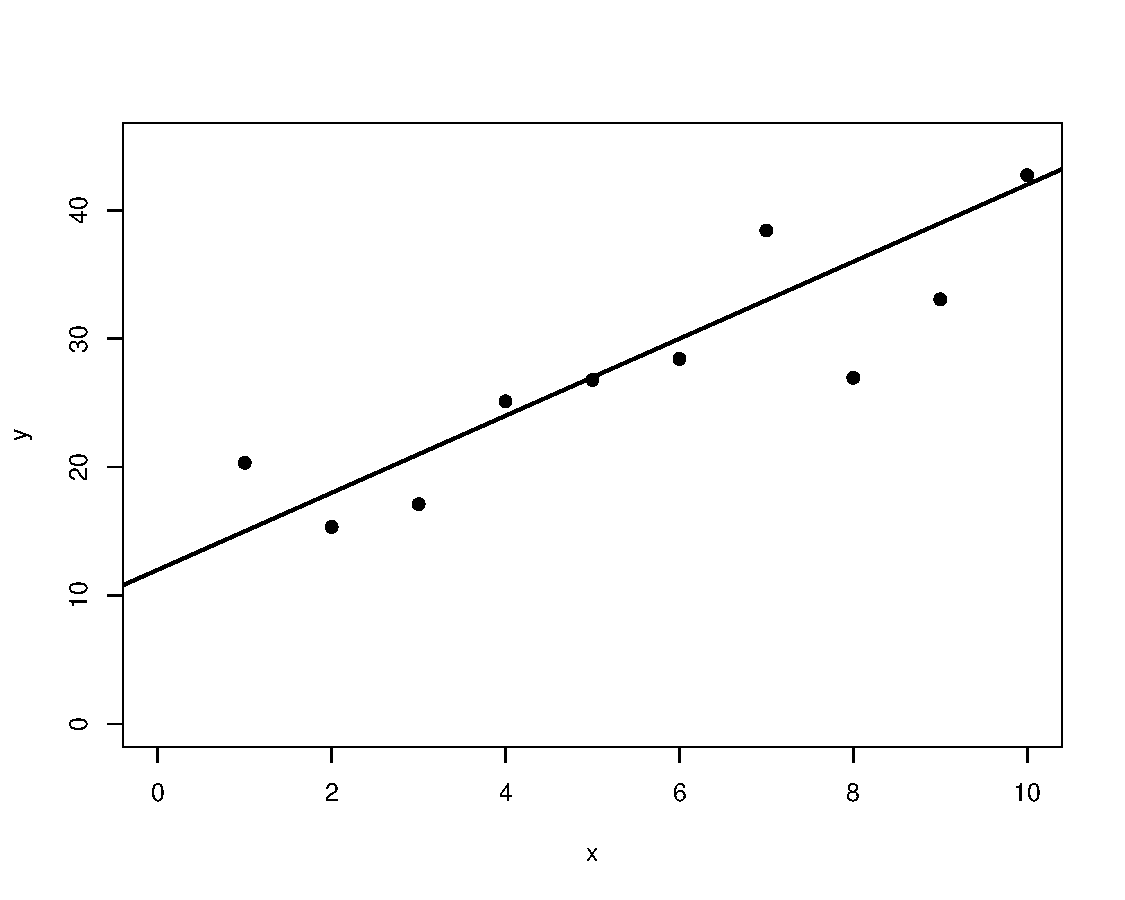
\includegraphics[width=0.7\linewidth]{figure/param4-1} 

\end{knitrout}


\end{frame}
%===============================================================================%


%===============================================================================%
\begin{frame}{Parâmetros do modelo de regressão}
\centering
$E[Y] = 12 + 3X$, \alert{$\beta _1 = 3$}
\vfill
$X=5$, $Y=27$; $X=6$, $Y=30$; $30 - 27 = 3$
\vfill
\begin{knitrout}
\definecolor{shadecolor}{rgb}{0.969, 0.969, 0.969}\color{fgcolor}
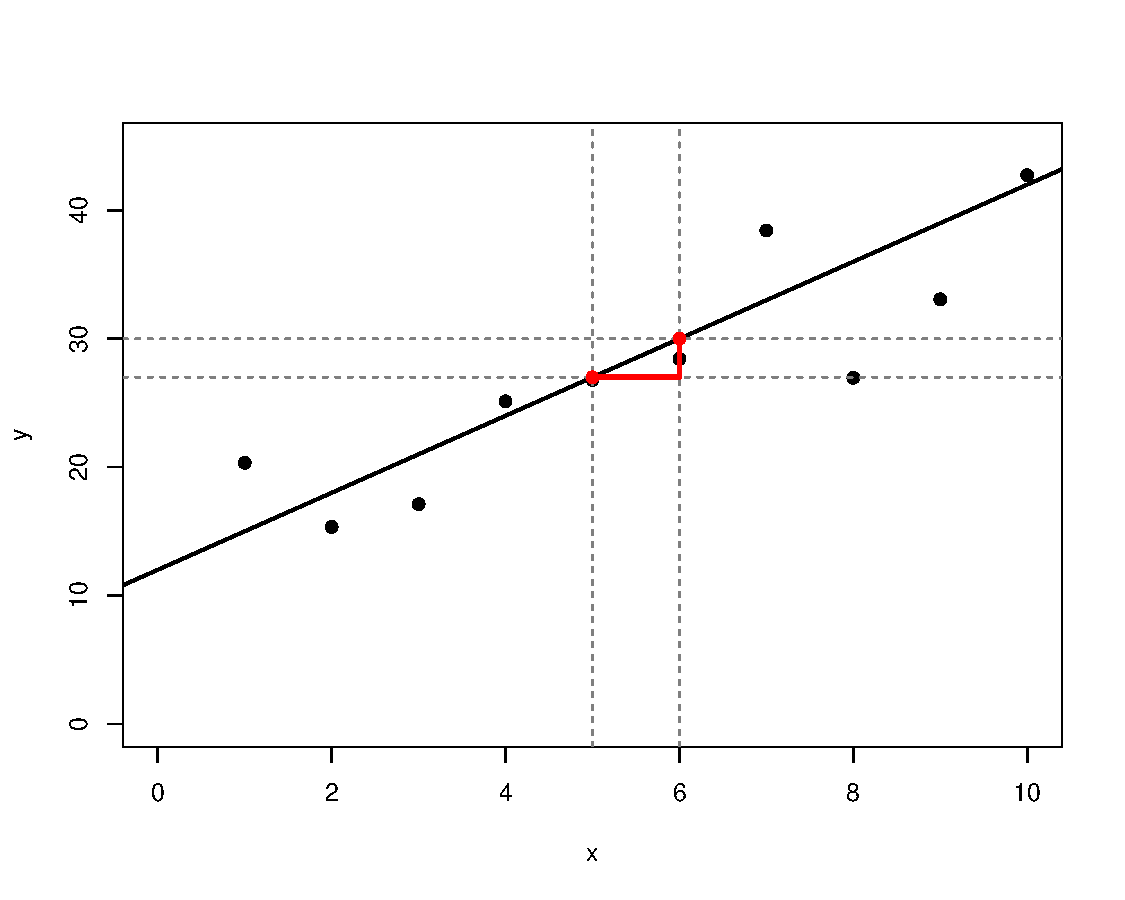
\includegraphics[width=0.7\linewidth]{figure/param5-1} 

\end{knitrout}


\end{frame}
%===============================================================================%

\section{Estimando o Modelo}




%===============================================================================%
\begin{frame}{Estimando o modelo de regressão}

Assim como outras estatísticas, assume-se que o modelo $E[Y] = \beta_0 + \beta _1 X + \varepsilon$ corresponde a uma população.\pause
\vfill
Ao tomarmos uma amostra de valores de $X$ e $Y$, queremos estimar o modelo $\hat Y = b_0 + b_1X + e$ \pause
\vfill 
Idealmente, gostaríamos de usar um método onde $\hat Y$, $b_0$, $b_1$ e $e$ sejam bons estimadores (não-tendenciosos) de $Y$, $\beta _0$, $\beta _1$ e $\varepsilon$. 

\end{frame}
%===============================================================================%


%===============================================================================%
\begin{frame}{Estimando o modelo de regressão}

Para isso, podemos usar o método dos \textbf{Mínimos Quadrados Comuns (\emph{Ordinary Least Squares, OLS})}. Este método considera as diferenças entre cada valor $Y_i$ e seu valor esperado $E[Y_i]$:
\vfill
\begin{equation*}
Y_i - E[Y_i] = Y_i - (\beta _0 + \beta_1 X_i) \pause
\end{equation}
\vfill
Como no caso das variâncias, estamos interessados no quadrado destas diferenças, para que elas não se cancelem: \pause
\vfill
\begin{equation*}
Q = \sum_{i=1}^{n}(Y_i - (\beta _0 + \beta_1 X_i))^2
\end{equation*}
\vfill
\end{frame}
%===============================================================================%


%===============================================================================%
\begin{frame}{Estimando o modelo de regressão}

De acordo com a formulação do método OLS, os melhores estimadores de $ \beta _0$ e $\beta _1$ são os valores $b_0$ e $b_1$ que minimizam o critério Q para as amostras obtidas. \pause
\vfill
\begin{columns}[c]

\column{0.5\linewidth}

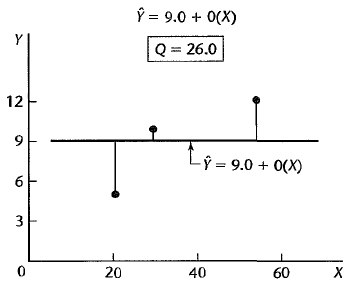
\includegraphics[width=1\linewidth]{Fig_[3].jpg} \pause

\column{0.5\linewidth}

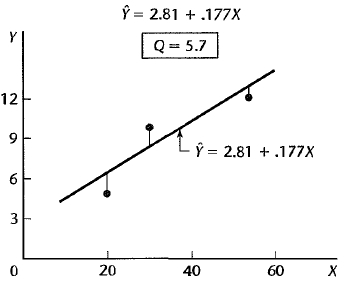
\includegraphics[width=1\linewidth]{Fig_[4].jpg}

\end{columns}

\end{frame}
%===============================================================================%

%===============================================================================%
\begin{frame}{Estimando o modelo de regressão}

Os estimadores $b_0$ e $b_1$ que satisfazem o critério de mínimos quadrados podem ser determinados de duas maneiras: \pause
\vfill
\begin{itemize}
  \item Numericamente, através de procedimentos de busca  computacional.
  \vfill
  \item Analiticamente. Este método só funciona para Modelos Lineares Gerais. 
\end{itemize}
\vfill \pause
Para a regressão simples, o método analítico nos dá:
\vfill
\begin{columns}[c]
\column{0.5\linewidth}
\begin{equation*}
b_0 = \bar Y - b_1 \bar X
\end{equation*}
\column{0.5\linewidth}
\begin{equation*}
b_1 = \frac{\sum(X_i - \bar X)(Y_i - \bar Y)}{\sum(X_i - \bar X)^2}
\end{equation*}  
\end{columns}  
\vfill
\tiny{Ver Kutner et al. (2005) Applied Linear Statistical Models. 5th ed. McGraw Hill. para a dedução analítica. I know you want to.}

\end{frame}
%===============================================================================%



%===============================================================================%
\begin{frame}{Exemplo}

\begin{columns}[t]

\column{0.5\linewidth}


\begin{tiny}
\begin{table}[ht]
\centering
\begin{tabular}{rrrr}
  \hline
  $X$ & $Y$ & $(X - \bar X)(Y - \bar Y)$ & $(X - \bar X)^2$ \\ 
  \hline
  9.09 & 12.10 & 14.97 & 24.14 \\ 
  4.82 & 7.28 & -1.14 & 0.42 \\ 
  2.53 & 7.25 & 2.98 & 2.71 \\ 
  7.28 & 12.76 & 11.51 & 9.66 \\ 
  1.66 & 8.92 & 0.35 & 6.35 \\ 
  2.64 & 8.30 & 1.16 & 2.35 \\ 
  6.11 & 11.22 & 4.17 & 3.74 \\ 
  3.88 & 12.96 & -1.16 & 0.09 \\ 
  4.79 & 9.71 & 0.41 & 0.38 \\ 
  3.66 & 10.34 & -0.66 & 0.26 \\ 
  3.47 & 9.44 & -0.27 & 0.49 \\ 
  0.70 & 1.97 & 24.65 & 12.12 \\ 
  9.12 & 15.51 & 31.94 & 24.49 \\ 
  2.76 & 5.56 & 4.93 & 1.99 \\ 
  0.12 & 2.52 & 26.52 & 16.46 \\ 
   \hline
  $\bar X$ & $\bar Y$ & $\sum(X - \bar X)(Y - \bar Y)$ & $\sum(X - \bar X)^2$\\
  \hline
  4.18 & 9.06 & 120.35 &  105.66 \\
  \hline
\end{tabular}
\end{table}
\end{tiny}

\column{0.5\linewidth}

\begin{equation*}
b_1 = \frac{\sum(X_i - \bar X)(Y_i - \bar Y)}{\sum(X_i - \bar X)^2}
\end{equation*}  \pause
\vfill
\begin{equation*}
b_1 = \frac{120.35}{105.66}
\end{equation*}  \pause
\vfill
\begin{equation*}
b_1 = 1.14
\end{equation*} 
\vfill
\end{columns}  


\end{frame}
%===============================================================================%

%===============================================================================%
\begin{frame}{Exemplo}

\begin{columns}[c]

\column{0.5\linewidth}

\begin{tiny}
\begin{table}[ht]
\centering
\begin{tabular}{rrrr}
  \hline
  $X$ & $Y$ & $(X - \bar X)(Y - \bar Y)$ & $(X - \bar X)^2$ \\ 
  \hline
  9.09 & 12.10 & 14.97 & 24.14 \\ 
  4.82 & 7.28 & -1.14 & 0.42 \\ 
  2.53 & 7.25 & 2.98 & 2.71 \\ 
  7.28 & 12.76 & 11.51 & 9.66 \\ 
  1.66 & 8.92 & 0.35 & 6.35 \\ 
  2.64 & 8.30 & 1.16 & 2.35 \\ 
  6.11 & 11.22 & 4.17 & 3.74 \\ 
  3.88 & 12.96 & -1.16 & 0.09 \\ 
  4.79 & 9.71 & 0.41 & 0.38 \\ 
  3.66 & 10.34 & -0.66 & 0.26 \\ 
  3.47 & 9.44 & -0.27 & 0.49 \\ 
  0.70 & 1.97 & 24.65 & 12.12 \\ 
  9.12 & 15.51 & 31.94 & 24.49 \\ 
  2.76 & 5.56 & 4.93 & 1.99 \\ 
  0.12 & 2.52 & 26.52 & 16.46 \\ 
   \hline
  $\bar X$ & $\bar Y$ & $\sum(X - \bar X)(Y - \bar Y)$ & $\sum(X - \bar X)^2$\\
  \hline
  4.18 & 9.06 & 120.35 &  105.66 \\
  \hline
\end{tabular}
\end{table}
\end{tiny}

\column{0.5\linewidth}

\begin{equation*}
b_0 = \bar Y - b_1 \bar X
\end{equation*} \pause
\vfill
\begin{equation*}
b_0 = 9.06 - 1.14 \times 4.18
\end{equation*}  \pause
\vfill
\begin{equation*}
b_0 = 9.06 - 4.77
\end{equation*}  \pause 
\vfill
\begin{equation*}
b_0 = 4.3
\end{equation*} 
\vfill
\end{columns}  


\end{frame}
%===============================================================================%



%===============================================================================%
\begin{frame}
\centering
$ \hat Y = 4.3 + 1.14X$
\vfill
\begin{knitrout}
\definecolor{shadecolor}{rgb}{0.969, 0.969, 0.969}\color{fgcolor}
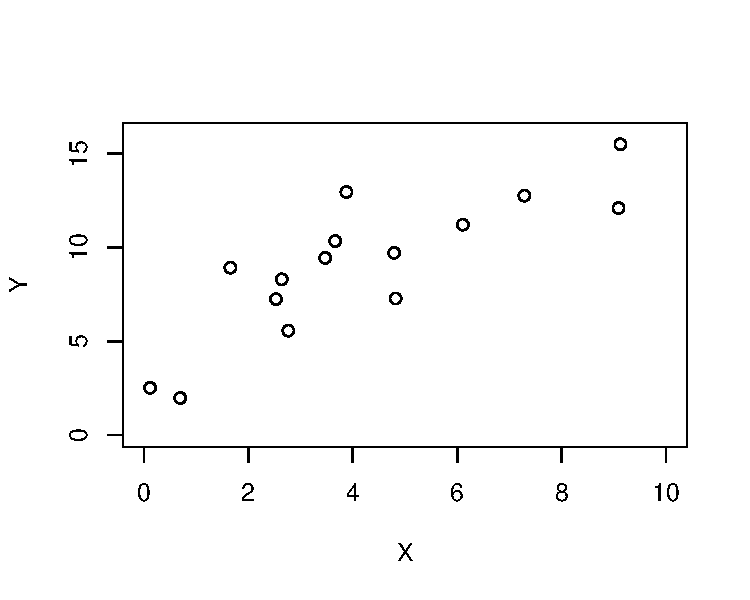
\includegraphics[width=0.8\linewidth]{figure/plotexample1-1} 

\end{knitrout}

\end{frame}
%===============================================================================%

%===============================================================================%
\begin{frame}
\centering
$ \hat Y = 4.3 + 1.14X$
\vfill
\begin{knitrout}
\definecolor{shadecolor}{rgb}{0.969, 0.969, 0.969}\color{fgcolor}
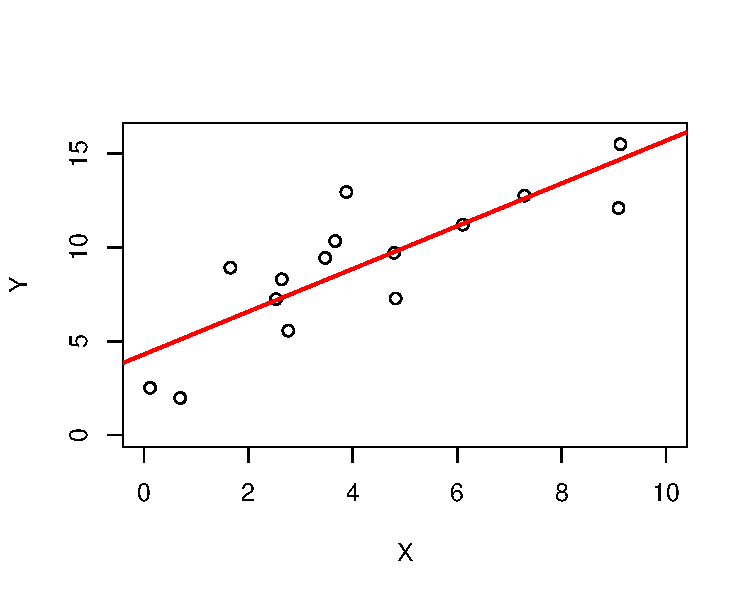
\includegraphics[width=0.8\linewidth]{figure/plotexample2-1} 

\end{knitrout}

\end{frame}
%===============================================================================%


%===============================================================================%
\begin{frame}{Os resíduos}

Olhando a nossa equação estimada, será que está faltando alguma coisa?
\vfill
\begin{equation*}
\hat Y_i = b_0 + b_1 X_i 
\end{equation} \pause
\vfill
Onde está o termo de erro estimado, $e$? 
\vfill
\begin{equation*}
\hat Y_i = b_0 + b_1 X_i + e
\end{equation*}
\vfill
\end{frame}
%===============================================================================%


%===============================================================================%
\begin{frame}{Os resíduos}

Os erros estimados $e_i$ são chamados de \textbf{resíduos} da regressão:
\vfill
\begin{equation*}
\alert{e_i} = Y_i - \textcolor{blue}{\hat Y_i} 
\end{equation} 
\vfill
\centering
\begin{knitrout}
\definecolor{shadecolor}{rgb}{0.969, 0.969, 0.969}\color{fgcolor}
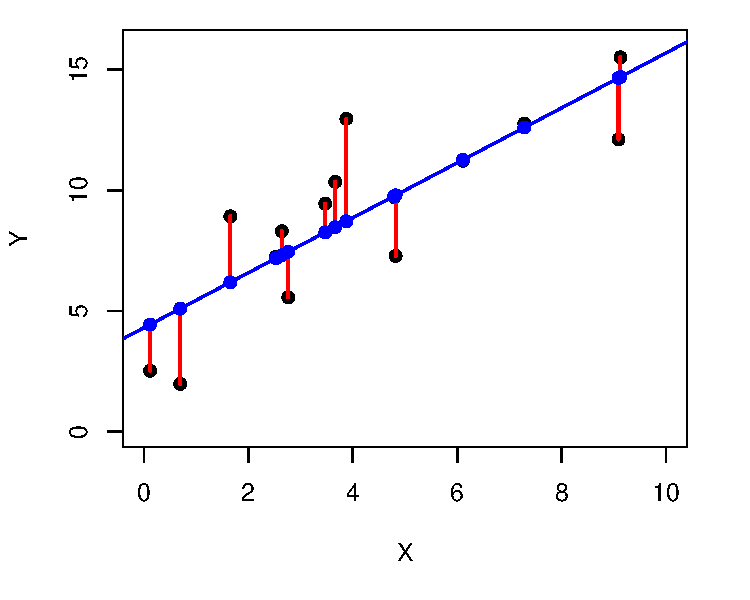
\includegraphics[width=0.6\linewidth]{figure/residplot-1} 

\end{knitrout}
\vfill
\end{frame}
%===============================================================================%

%===============================================================================%
\begin{frame}{Propriedades do modelo de regressão}

\begin{enumerate}
  \item A soma dos resíduos é zero : $\sum e_i = 0$ \pause
  \vfill
  \item A soma dos quadrados dos resíduos, $\sum e_i^2$ é um mínimo \pause
  \vfill
  \item A soma dos valores observados $Y_i$ é igual a soma dos valores ajustados $\hat Y_i$ \pause
  \vfill
  \item A soma dos resíduos ponderada pelos valores de $X_i$ é zero: $\sum X_i e_i = 0$ \pause
  \vfill
  \item Devido a 1) e 4), a soma dos resíduos ponderada pelos valores de $\hat Y_i$ também é zero: \sum \hat Y_i e_i = 0$ \pause
  \vfill
  \item \textbf{A reta de regressão sempre passa pelo ponto ($\bar X$,$\bar Y$)}
\end{enumerate}

\end{frame}
%===============================================================================%

\section{Estimando a Variância do Modelo}


%===============================================================================%
\begin{frame}{Estimando a variância de uma população}

\begin{small}
A variância de $\varepsilon$ também precisa ser estimada, a fim de caracterizar a distribuição de probabilidade de $Y$ para cada nível de $X$, e permitir inferências sobre o modelo. \pause
\vfill
\textbf{Relembrando:} A variância de uma população $Y$ ($\sigma ^2$) pode ser estimada pela variância de uma amostra ($s^2$), através da \textbf{soma dos quadrados} dos desvios de $Yi$ a partir de $\bar Y$:
\vfill
\begin{equation*}
\sum_{i-1}^{n}(Y_i - \bar Y)^2
\end{equation*}
\vfill \pause
Para obter $s^2$, nós dividimos a soma dos quadrados pelos graus de liberdade associados com essa soma:
\begin{equation*}
s^2 =\frac{\sum_{i-1}^{n}(Y_i - \bar Y)^2}{n-1}
\end{equation*}
\end{small}

\end{frame}
%===============================================================================%

%===============================================================================%
\begin{frame}{Estimando a variância do modelo}

\begin{small}
Uma das pressuposições do modelo de regressão linear é que $s^2$ é constante. A única diferença para a variância comum é que, no modelo, a distribuição de $Y_i$ varia de acordo com o nível de $X$, então os desvios são calculados em relação a $\hat Y$, e não $\bar Y$: \pause
\vfill
\begin{equation*}
Y_i - \hat Y = e_i
\end{equation*}
\vfill \pause
E a soma do quadrado destes valores é chamada de \textbf{Soma dos Quadrados dos Erros/Resíduos} ($SQ_{res}$\footnote{\tiny{Essa nomenclatura varia, vejam exatamente quem é quem ao ler um livro/artigo}}):
\begin{equation*}
SQ_{res} =\sum_{i-1}^{n}(Y_i - \hat Y)^2 = \sum_{i-1}^{n}e_i^2
\end{equation*}
\end{small}

\end{frame}
%===============================================================================%


%===============================================================================%
\begin{frame}{Estimando a variância do modelo}

\begin{small}
A $SQ_{res}$ tem $n-2$ graus de liberdade, por que dois graus são perdidos estimando-se $\beta _0$ e $\beta_1$. Assim, temos que $s^2$ é:
\vfill 
\begin{equation*}
s^2 = MQ_{res} = \frac{SQ_{res}}{n-2} = \frac{\sum(Y_i - \hat Y)^2}{n-2} = \frac{\sum e_i^2}{n-2}
\end{equation*}
\end{small}
\vfill
A divisão por $n - 2$ é apenas uma normalização para proporção. Mas não é necessária para entender a quantidade de variação. 
\end{frame}
%===============================================================================%

%===============================================================================%
\begin{frame}[fragile]

\begin{columns}[t]

\column{0.5\linewidth}

\begin{knitrout}\tiny
\definecolor{shadecolor}{rgb}{0.969, 0.969, 0.969}\color{fgcolor}\begin{kframe}
\begin{alltt}
\hlkwd{set.seed}\hlstd{(}\hlnum{1979}\hlstd{)}
\hlstd{x} \hlkwb{<-} \hlkwd{runif}\hlstd{(}\hlnum{15}\hlstd{,}\hlnum{1}\hlstd{,}\hlnum{10}\hlstd{)}
\hlstd{y} \hlkwb{<-} \hlnum{2} \hlopt{+} \hlnum{3}\hlopt{*}\hlstd{x} \hlopt{+} \hlkwd{rnorm}\hlstd{(}\hlnum{15}\hlstd{,}\hlnum{0}\hlstd{,}\hlnum{3}\hlstd{)}
\hlstd{m} \hlkwb{<-} \hlkwd{lm}\hlstd{(y} \hlopt{~} \hlstd{x)}
\hlkwd{summary}\hlstd{(m)}
\end{alltt}
\begin{verbatim}
## 
## Call:
## lm(formula = y ~ x)
## 
## Residuals:
##    Min     1Q Median     3Q    Max 
## -3.742 -2.281  0.078  1.308  5.090 
## 
## Coefficients:
##             Estimate Std. Error t value Pr(>|t|)    
## (Intercept)   4.7349     1.5059   3.144  0.00776 ** 
## x             2.7854     0.2828   9.848 2.15e-07 ***
## ---
## Signif. codes:  0 '***' 0.001 '**' 0.01 '*' 0.05 '.' 0.1 ' ' 1
## 
## Residual standard error: 2.617 on 13 degrees of freedom
## Multiple R-squared:  0.8818,	Adjusted R-squared:  0.8727 
## F-statistic: 96.98 on 1 and 13 DF,  p-value: 2.149e-07
\end{verbatim}
\end{kframe}
\end{knitrout}

\column{0.5\linewidth}

\begin{knitrout}\tiny
\definecolor{shadecolor}{rgb}{0.969, 0.969, 0.969}\color{fgcolor}\begin{kframe}
\begin{alltt}
\hlstd{ypred} \hlkwb{<-} \hlkwd{predict}\hlstd{(m)}
\hlkwd{plot}\hlstd{(x,y,}\hlkwc{xlim}\hlstd{=}\hlkwd{c}\hlstd{(}\hlnum{0}\hlstd{,}\hlnum{10}\hlstd{),}\hlkwc{ylim}\hlstd{=}\hlkwd{c}\hlstd{(}\hlnum{0}\hlstd{,}\hlnum{40}\hlstd{))}
\hlkwd{abline}\hlstd{(m)}
\hlkwd{segments}\hlstd{(}\hlkwc{x0}\hlstd{=x,} \hlkwc{x1}\hlstd{=x,}\hlkwc{y0}\hlstd{=ypred,}\hlkwc{y1}\hlstd{=y,}
         \hlkwc{col}\hlstd{=}\hlstr{'red'}\hlstd{,}\hlkwc{lwd}\hlstd{=}\hlnum{2}\hlstd{)}
\end{alltt}
\end{kframe}
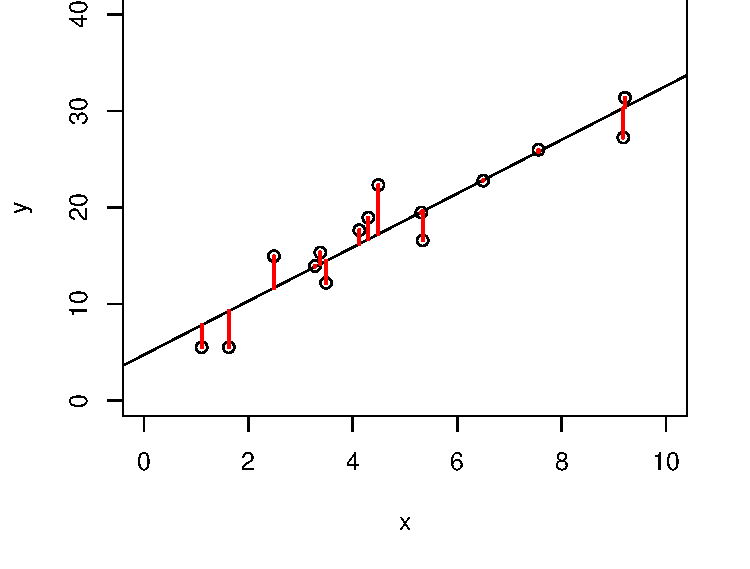
\includegraphics[width=1\linewidth]{figure/esd3plot-1} 

\end{knitrout}

\end{columns}

\end{frame}
%===============================================================================%

%===============================================================================%
\begin{frame}[fragile]

\begin{columns}[t]

\column{0.5\linewidth}

\begin{knitrout}\tiny
\definecolor{shadecolor}{rgb}{0.969, 0.969, 0.969}\color{fgcolor}\begin{kframe}
\begin{alltt}
\hlkwd{set.seed}\hlstd{(}\hlnum{1979}\hlstd{)}
\hlstd{x} \hlkwb{<-} \hlkwd{runif}\hlstd{(}\hlnum{15}\hlstd{,}\hlnum{1}\hlstd{,}\hlnum{10}\hlstd{)}
\hlstd{y} \hlkwb{<-} \hlnum{2} \hlopt{+} \hlnum{3}\hlopt{*}\hlstd{x} \hlopt{+} \hlkwd{rnorm}\hlstd{(}\hlnum{15}\hlstd{,}\hlnum{0}\hlstd{,}\hlnum{10}\hlstd{)}
\hlstd{m} \hlkwb{<-} \hlkwd{lm}\hlstd{(y} \hlopt{~} \hlstd{x)}
\hlkwd{summary}\hlstd{(m)}
\end{alltt}
\begin{verbatim}
## 
## Call:
## lm(formula = y ~ x)
## 
## Residuals:
##      Min       1Q   Median       3Q      Max 
## -12.4732  -7.6035   0.2601   4.3598  16.9658 
## 
## Coefficients:
##             Estimate Std. Error t value Pr(>|t|)  
## (Intercept)  11.1165     5.0196   2.215   0.0453 *
## x             2.2847     0.9428   2.423   0.0307 *
## ---
## Signif. codes:  0 '***' 0.001 '**' 0.01 '*' 0.05 '.' 0.1 ' ' 1
## 
## Residual standard error: 8.722 on 13 degrees of freedom
## Multiple R-squared:  0.3112,	Adjusted R-squared:  0.2582 
## F-statistic: 5.872 on 1 and 13 DF,  p-value: 0.03072
\end{verbatim}
\end{kframe}
\end{knitrout}

\column{0.5\linewidth}

\begin{knitrout}\tiny
\definecolor{shadecolor}{rgb}{0.969, 0.969, 0.969}\color{fgcolor}\begin{kframe}
\begin{alltt}
\hlstd{ypred} \hlkwb{<-} \hlkwd{predict}\hlstd{(m)}
\hlkwd{plot}\hlstd{(x,y,}\hlkwc{xlim}\hlstd{=}\hlkwd{c}\hlstd{(}\hlnum{0}\hlstd{,}\hlnum{10}\hlstd{),}\hlkwc{ylim}\hlstd{=}\hlkwd{c}\hlstd{(}\hlnum{0}\hlstd{,}\hlnum{40}\hlstd{))}
\hlkwd{abline}\hlstd{(m)}
\hlkwd{segments}\hlstd{(}\hlkwc{x0}\hlstd{=x,} \hlkwc{x1}\hlstd{=x,}\hlkwc{y0}\hlstd{=ypred,}\hlkwc{y1}\hlstd{=y,}
         \hlkwc{col}\hlstd{=}\hlstr{'red'}\hlstd{,}\hlkwc{lwd}\hlstd{=}\hlnum{2}\hlstd{)}
\end{alltt}
\end{kframe}
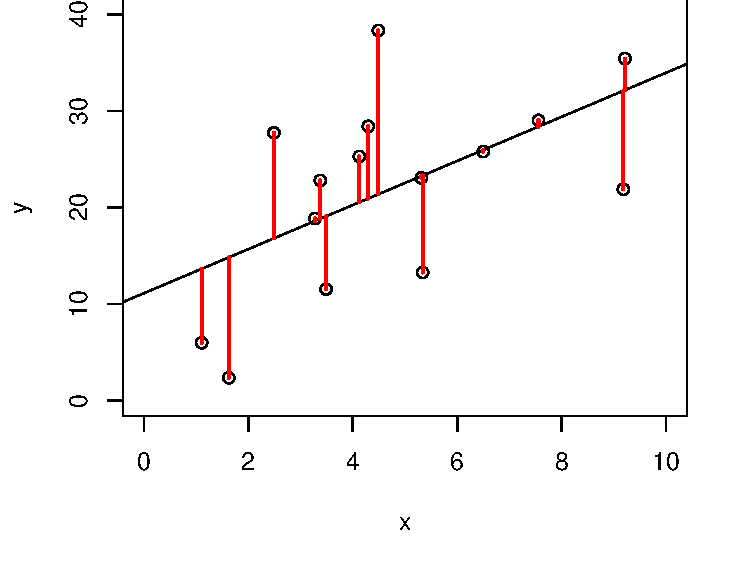
\includegraphics[width=1\linewidth]{figure/esd10plot-1} 

\end{knitrout}

\end{columns}

\end{frame}
%===============================================================================%

%===============================================================================%
\begin{frame}{Partição da variância e o Coeficiente de Determinação}

Agora, já sabemos como estimar todos os componentes do modelo:  $\hat Y$, $b_0$, $b_1$, e $s^2$. O que mais precisamos? \pause
\vfill
\begin{itemize}
  \item De um método para avaliar a qualidade da estimação \pause
  \vfill
  \only<3>{\item De um método para avaliar o ajuste do modelo}
  \end{itemize}

\end{frame}
%===============================================================================%


%===============================================================================%
\begin{frame}{Partição da variância e o Coeficiente de Determinação}

\begin{itemize}
\item Como vimos antes, $SQ_{res}$ nos dá a variancia dos resíduos. \pause
\vfill
\item A variância contida em $SQ_{res}$ é a quantidade de variação que é aleatória, e não pôde ser capturada pelo modelo \pause
\vfill
\item Essa variação é uma parte da variância total de $Y$ (Soma dos Quadrados Totais, $SQ_{tot}$) \pause
\vfill 
\item Podemos então definir a "variância explicada pelo modelo", como sendo a diferença entre a variância total de $Y$ ($SQ_{tot}$), e a variância dos resíduos ($SQ_{res}$):
\end{itemize}
\vfill
\begin{equation*}
  SQ_{reg} =  SQ_{tot} - SQ_{res}
\end{equation*}

\end{frame}
%===============================================================================%


%===============================================================================%
\begin{frame}{Partição da variância e o Coeficiente de Determinação}

Essa partição pode ser melhor entendida ao se considerarem duas situações extremas: \pause
\vfill

\begin{itemize}
  \item Se todos os valores de $Y$ caíssem exatamente em cima da reta, $SQ_{res} = 0$, e $SQ_{reg} = SQ_{tot}$ \pause
  \vfill
  \item Se não há relação entre $X$ e $Y$, $\beta _1 = 0$, e $Y = \beta_0 + \varepsilon$. Nesse caso, $Y \sim N(\beta _0,\sigma)$, e $SQ_{tot} = SQ_{res}$  \pause
\end{itemize}

\end{frame}
%===============================================================================%

%===============================================================================%
\begin{frame}[fragile]

\begin{columns}[c]

\column{0.5\linewidth}

\begin{knitrout}\tiny
\definecolor{shadecolor}{rgb}{0.969, 0.969, 0.969}\color{fgcolor}\begin{kframe}
\begin{alltt}
\hlkwd{set.seed}\hlstd{(}\hlnum{1979}\hlstd{)}
\hlstd{x} \hlkwb{<-} \hlkwd{runif}\hlstd{(}\hlnum{15}\hlstd{,}\hlnum{1}\hlstd{,}\hlnum{10}\hlstd{)}
\hlstd{y} \hlkwb{<-} \hlnum{2} \hlopt{+} \hlnum{3}\hlopt{*}\hlstd{x}
\hlstd{m} \hlkwb{<-} \hlkwd{lm}\hlstd{(y} \hlopt{~} \hlstd{x)}
\hlkwd{anova}\hlstd{(m)[}\hlstr{"Sum Sq"}\hlstd{]}
\end{alltt}
\begin{verbatim}
##           Sum Sq
## x         770.26
## Residuals   0.00
\end{verbatim}
\begin{alltt}
\hlkwd{var}\hlstd{(y)}\hlopt{*}\hlstd{(}\hlnum{15}\hlopt{-}\hlnum{1}\hlstd{)}
\end{alltt}
\begin{verbatim}
## [1] 770.2641
\end{verbatim}
\end{kframe}
\end{knitrout}

\begin{knitrout}\tiny
\definecolor{shadecolor}{rgb}{0.969, 0.969, 0.969}\color{fgcolor}
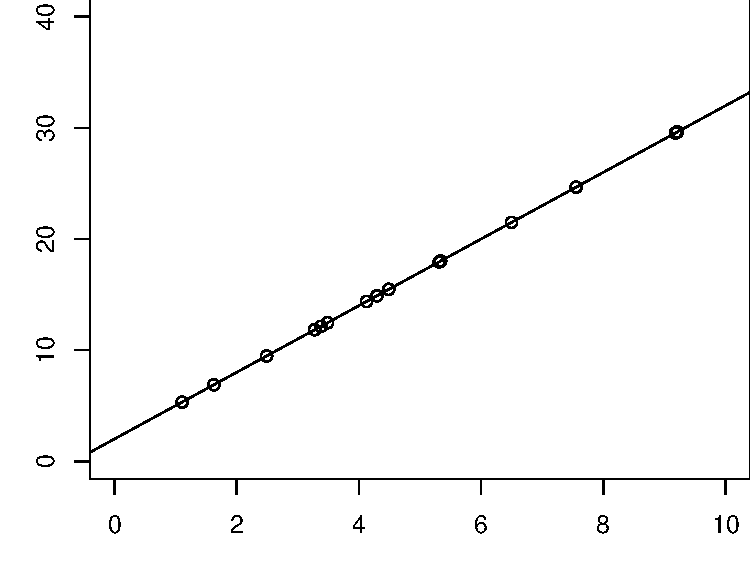
\includegraphics[width=0.7\linewidth]{figure/sse0plot-1} 

\end{knitrout}


\column{0.5\linewidth}

\begin{knitrout}\tiny
\definecolor{shadecolor}{rgb}{0.969, 0.969, 0.969}\color{fgcolor}\begin{kframe}
\begin{alltt}
\hlkwd{set.seed}\hlstd{(}\hlnum{1979}\hlstd{)}
\hlstd{x} \hlkwb{<-} \hlkwd{runif}\hlstd{(}\hlnum{15}\hlstd{,}\hlnum{1}\hlstd{,}\hlnum{10}\hlstd{)}
\hlstd{y} \hlkwb{<-} \hlnum{2} \hlopt{+} \hlkwd{rnorm}\hlstd{(}\hlnum{15}\hlstd{,}\hlnum{0}\hlstd{,}\hlnum{3}\hlstd{)}
\hlstd{m} \hlkwb{<-} \hlkwd{lm}\hlstd{(y} \hlopt{~} \hlstd{x)}
\hlkwd{anova}\hlstd{(m)[}\hlstr{"Sum Sq"}\hlstd{]}
\end{alltt}
\begin{verbatim}
##           Sum Sq
## x          3.941
## Residuals 89.006
\end{verbatim}
\begin{alltt}
\hlkwd{var}\hlstd{(y)}\hlopt{*}\hlstd{(}\hlnum{15}\hlopt{-}\hlnum{1}\hlstd{)}
\end{alltt}
\begin{verbatim}
## [1] 92.94772
\end{verbatim}
\end{kframe}
\end{knitrout}

\begin{knitrout}\tiny
\definecolor{shadecolor}{rgb}{0.969, 0.969, 0.969}\color{fgcolor}
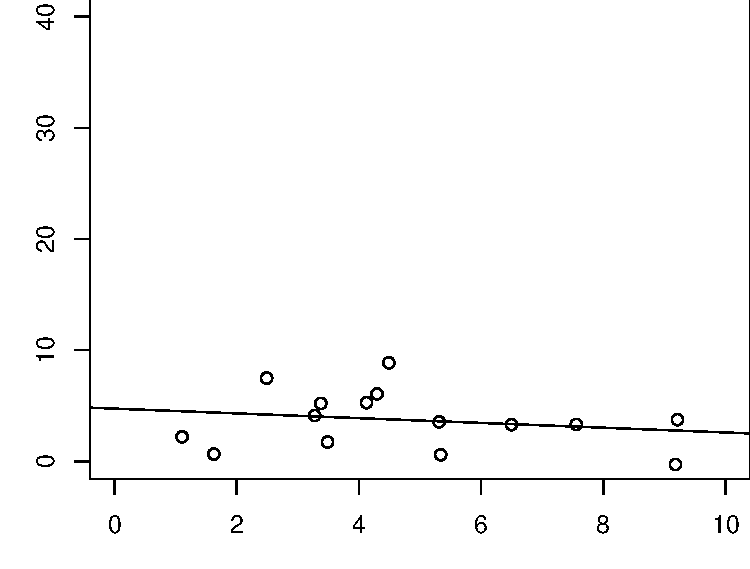
\includegraphics[width=0.7\linewidth]{figure/ssr0plot-1} 

\end{knitrout}

\end{columns}

\end{frame}
%===============================================================================%

%===============================================================================%
\begin{frame}{Coeficiente de Determinação}

\begin{columns}[c]

\column{0.3\linewidth}


\includegraphics[width=0.9\linewidth]{heman.jpg}

\column{0.8\linewidth}

A partir desta formulação, chegamos ao \textbf{Coeficiente de Determinação ($R^2$)}: 
\vfill
\begin{equation*}
R^2 = \frac{SQ_{reg}}{SQ_{tot}} = \frac{SQ_{reg}}{SQ_{reg}+SQ_{res}}
\end{equation*} \pause
\vfill
Como podemos interpretar o valor de $R^2$? \pause
\vfill

$R^2$ nos dá a proporção da variância total de $Y$ explicada pelo modelo de regressão

\bigskip

\scriptsize{* $r^2$ se refere a um modelo simples, e $R^2$ a um modelo multivariado.}

\end{columns}

\end{frame}
%===============================================================================%


%===============================================================================%
\begin{frame}{Em resumo}
\setbeamercovered{transparent}

\begin{itemize}

\item Um modelo de \textbf{regressão linear} estima uma relação estatística entre \textbf{$X$} e \textbf{$Y$}, através de coeficientes lineares \textbf{$\beta$} \pause
\vfill
\item Esta relação é caracterizada por uma \textbf{co-variação} entre os níveis de $X$ e $E[Y]$ \pause
\vfill
\item A existência de co-variação não implica em \textbf{causalidade} \pause
\vfill
\item A variância de $Y$ não capturada pelo modelo constitui o \textbf{erro da regressão} ($\varepsilon$) \pause
\vfill
\item A \textbf{variância de} \textbf{$Y_i$} a cada nível de $X$ é dada pela variância de $\varepsilon$ \pause
\vfill
\item A \textbf{variância total} de \textbf{$Y$} é dada pela variância de $\varepsilon$ + a relação $\beta _0 + \beta _1 X$ 
\vfill
\end{itemize}
\vfill
\end{frame}
%===============================================================================%

%===============================================================================%
\begin{frame}{Em resumo}
\setbeamercovered{transparent}

\begin{itemize}

\item Os coeficientes $\beta _0$ e $\beta _1$ determinam o \textbf{intercepto} e a \textbf{inclinação da reta} \pause
\vfill
\item A reta de regressão ($\hat Y = b_0 + b_1X + e$) é estimada pelo método de \textbf{mínimos quadrados}, que busca minizar Soma dos Quadrados dos Erros ($SQ_{res}$) \pause
\vfill
\item A partir da diferença entre $SQ_{res}$ e a Soma dos Quadrados Totais ($SQ_{tot} = Var[Y]$), podemos estimar a Soma dos Quadrados da Regressão ($SQ_{reg}$) \pause
\vfill
\item A relação $\frac{SQ_{reg}}{SQ_{tot}}$ é chamada de $R^2$, e nos diz a proporção da variância total de $Y$ explicada pelo modelo$
\vfill
\end{itemize}

\end{frame}
%===============================================================================%


%===============================================================================%
\begin{frame}[fragile]

Interpretando o output do modelo de regressão no R \dots até agora.

\begin{knitrout}\tiny
\definecolor{shadecolor}{rgb}{0.969, 0.969, 0.969}\color{fgcolor}\begin{kframe}
\begin{verbatim}
## 
## Call:
## lm(formula = y ~ x)
## 
## Residuals:
##     Min      1Q  Median      3Q     Max 
## -7.7244 -3.9253  0.2196  3.5752  7.5188 
## 
## Coefficients:
##             Estimate Std. Error t value Pr(>|t|)    
## (Intercept)   0.3632     2.0016   0.181    0.858    
## x             3.3127     0.2058  16.099 3.93e-12 ***
## ---
## Signif. codes:  0 '***' 0.001 '**' 0.01 '*' 0.05 '.' 0.1 ' ' 1
## 
## Residual standard error: 4.81 on 18 degrees of freedom
## Multiple R-squared:  0.9351,	Adjusted R-squared:  0.9315 
## F-statistic: 259.2 on 1 and 18 DF,  p-value: 3.925e-12
\end{verbatim}
\end{kframe}
\end{knitrout}

\end{frame}
%===============================================================================%

\end{document}
